\documentclass[masterthesis]{fer}
% Add the option upload to generate the final version which is uploaded to FERWeb
% Dodaj opciju upload za generiranje konačne verzije koja se učitava na FERWeb


\usepackage{blindtext}


%--- THESIS INFORMATION / PODACI O RADU ----------------------------------------

% Title in English / Naslov na engleskom jeziku
\title{Uncomputable Computablity}

% Title in Croatian / Naslov na hrvatskom jeziku
\naslov{Neizračunljiva izračunljivost}

% Thesis number / Broj rada
\brojrada{1234}

% Author / Autor
\author{Ferko Ferovac}

% Mentor 
\mentor{Prof.\@ Baltazar}

% Date in English / Datum rada na engleskom jeziku
\date{June, 2021}

% Date in Croatian / Datum rada na hrvatskom jeziku
\datum{lipanj, 2021.}

%-------------------------------------------------------------------------------


\begin{document}


% Titlepage is automatically generated / Naslovnica se automatski generira
\maketitle


%--- THESIS ASSIGNMENT / ZADATAK -----------------------------------------------

% Thesis assignment is included from external file / Zadatak se ubacuje iz vanjske datoteke
% Enter the filename of the PDF downloaded from FERWeb / Upiši ime PDF datoteke preuzete s FERWeb-a
\zadatak{filename.pdf}


%--- ACKNOWLEDGMENT / ZAHVALE --------------------------------------------------

\begin{zahvale}
  % Write in the acknowledgment / Ovdje upišite zahvale
  Thanks for the tea...
\end{zahvale}


% Page numbering starts from here / Odovud započinje numeriranje stranica
\mainmatter


% Table of contents is automatically generated / Sadržaj se automatski generira
\tableofcontents


%--- INTRODUCTION / UVOD -------------------------------------------------------
\chapter{Introduction}
\label{chp:introduction}

Some of the works we will quote are \cite{6248073,6247753,ghiglia_pritt_phase_unwrapping,hartley2003multiple,4250461,123DCatch}.
The works are quoted here to test the referencing of a conference paper, of a journal paper, of a book, and of a webpage.

\begin{figure}[htb]
  \centering
  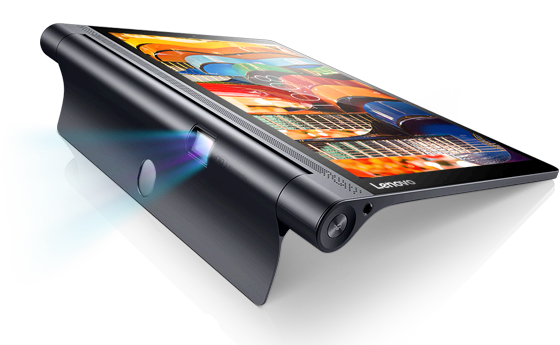
\includegraphics[width=0.38\linewidth]{Figures/lenovo_yoga_tab3_pro_front.png} 
  \caption{My first figure}
  \label{fig:firstfigure}
\end{figure}

Reference to the first figure \ref{fig:firstfigure} in the middle of a sentence, then before a comma \ref{fig:firstfigure}, and then at the end of a sentence \ref{fig:firstfigure}.
We have just tested if the command \verb|\ref| handles the following interpunction properly.

Now typeset one equation:
\begin{equation}
  \label{eq:firstequation}
  \int_{-\infty}^{+\infty}f(t)\,dt=F(\omega)
\end{equation}
The equation \eqref{eq:firstequation} is my first equation which defines a transform pair $f(t)\ufrek F(\omega)$ or $F(\omega)\uvrem f(t)$.


%-------------------------------------------------------------------------------
\chapter{Materials and Methods}
\label{sec:materialsandmethods}

\Blindtext


%-------------------------------------------------------------------------------
\chapter{Results and Discussion}
\label{sec:results_and_discussion}

\Blindtext


%--- CONCLUSION / ZAKLJUČAK ----------------------------------------------------
\chapter{Conclusion}
\label{chp:conclusion}

\blindtext


%--- REFERENCES / LITERATURA ---------------------------------------------------

% References are automatically generated from the supplied .bib file / Literatura se automatski generira iz zadane .bib datoteke
% Enter the name of the BibTeX file without .bib extension / Upiši ime BibTeX datoteke bez .bib nastavka
\bibliography{references}



%--- ABSTRACT / SAŽETAK --------------------------------------------------------

% Abstract in English
\begin{abstract}
  Enter the abstract in English.
  
  \blindtext 
\end{abstract}

\begin{keywords}
  the first keyword; the second keyword; the third keyword
\end{keywords}


% Sažetak na hrvatskom
\begin{sazetak}
  Unesite sažetak na hrvatskom.

  \blindtext
\end{sazetak}

\begin{kljucnerijeci}
  prva ključna riječ; druga ključna riječ; treća ključna riječ
\end{kljucnerijeci}



%--- APPENDIX / PRIVITCI -------------------------------------------------------

% All following chapters will be denoted with an appendix and a letter / Sva poglavlja koja slijede će biti označena slovom i riječi privitak
\backmatter

\chapter{The Code}

\Blindtext


\end{document}
